%
% section 3.1.7
%
\subsection{Αταξική Δρομολόγηση (CIDR), Υπερδικτύωση και Μάσκες Μεταβλητού Μήκους}

Με τη χρήση μάσκας δικτύου, τα τμήματα δικτύου και υπολογιστή καθορίζονται πλέον από αυτή, άρα οι τυποποιημένες κλάσεις παύουν να έχουν σημασία. Μπορούμε δηλ. να έχουμε διευθύνσεις όπως την παρακάτω:

IP: 10.14.28.10
Mask: 255.255.255.0

Σύμφωνα με αυτά που ξέρουμε από τις κλάσεις, η παραπάνω διεύθυνση θα άνηκε σε ένα δίκτυο κλάσης Α αν δεν υπήρχε η μάσκα. Όμως με τη συγκεκριμένη μάσκα, η διεύθυνση πλέον φαίνεται να αντιστοιχεί σε κλάση C. Στην πραγματικότητα, με τη χρήση της μάσκας δεν υπάρχουν πλέον κλάσεις και μπορούμε να έχουμε δίκτυα που δεν ανήκουν σε καμιά τυποποιημένη κλάση (σε αυτά η μάσκα περιέχει και τιμές διαφορετικές από 0 και 255).

Με αυτό τον τρόπο διευκολύνεται η διαδικασία της δρομολόγησης και της διαχείρισης των πινάκων δρομολόγησης από τους δρομολογητές (routers) IPv4.  Όλος ο χώρος διευθύνσεων αντιμετωπίζεται ως ενιαίος και χωρίς κλάσεις από τα πρωτόκολλα δρομολόγησης.  Η δρομολόγηση αυτή ονομάζεται \emph{αταξική} ή \emph{CIDR (Classless Internet Domain Routing)}.

Για παράδειγμα, σε μια εταιρεία με ανάγκες 1000 υπολογιστών, δεν θα δώσουμε πλέον ένα δίκτυο κλάσης B (με απώλεια των υπόλοιπων 64534 διευθύνσεων) αλλά τέσσερα συνεχόμενα δίκτυα κλάσης C. Τα δίκτυα αυτά ωστόσο θα τα αντιμετωπίζουμε ως ένα ενιαίο χώρο.

\begin{inthebox}
Στην προηγούμενη ενότητα, δίναμε ψηφία από το αναγνωριστικό του υπολογιστή στο αναγνωριστικό του δικτύου. Αυτό το ονομάσαμε \textbf{υποδικτύωση}. Εδώ θα δώσουμε ψηφία από το αναγνωριστικό δικτύου στο αναγνωριστικό του υπολογιστή και θα έχουμε \textbf{υπερδικτύωση}.

Στην υποδικτύωση,  χωρίζουμε ένα μεγαλύτερο δίκτυο σε μικρότερα κομμάτια. Στην υπερδικτύωση φτιάχνουμε ένα μεγαλύτερο δίκτυο ενώνοντας μικρότερα. Στο παράδειγμα μας θα ενώσουμε τέσσερα δίκτυα που κανονικά θα χαρακτηρίζονταν ως κλάσης C για ένα μεγαλύτερο δίκτυο που θα διαθέτει 1024 διευθύνσεις, θα μπορεί δηλ. να συνδέσει 1022 μηχανήματα.\\
\end{inthebox}

Για να βάλουμε 1000 μηχανήματα, θα χρειαστούμε 10 bit στο τμήμα υπολογιστή, αφού 2\textsuperscript{10}=1024. Άρα τα υπόλοιπα 22 bit θα αποτελέσουν το τμήμα δικτύου. Έχουμε δώσει δηλ. δύο παραπάνω bit στο τμήμα υπολογιστή σε σχέση με την τυποποιημένη κλάση C. Η νέα μας μάσκα θα είναι:

11111111.11111111.11111100.00000000 ή 255.255.252.0

Θεωρώντας π.χ. το δίκτυο 194.75.128.0/22, θα έχουμε τις παρακάτω διευθύνσεις:

\begin{center}
\fontsize{10}{12}
\ttfamily
\begin{tabular}{|c|c|c|c|c|c|c|}
\hline
    Α/Α              & 1η οκτάδα & 2η οκτάδα & \multicolumn{2}{c|}{3η οκτάδα} & 4η οκτάδα & Διευθύνσεις \\ \hline
\multirow{2}{*}{ΔΥ} & 11000010  & 01001011 & \multirow{2}{*}{100000}  & 00 & 00000000 & 194.75.128.0 \\ \cline{2-3} \cline{5-7} 
                  & 11000010 & 01001011 &                    & 11 & 11111111 & 194.75.131.255 \\ \hline
\end{tabular}
\normalfont
\end{center}

\begin{inthebox}
\textbf{Σημείωση:} Το παράδειγμα του βιβλίου χρησιμοποιεί διεύθυνση τύπου 192.Χ.Χ.Χ η οποία καθώς ξέρουμε χρησιμοποιείται για ιδιωτικά δίκτυα και δεν θα μας δίνονταν ποτέ ως περιοχή διευθύνσεων από IANA/ICANN.\\
\end{inthebox}
 
Δεν τίθεται εδώ θέμα υποδικτύωσης. Το δίκτυο είναι ενιαίο και είναι το\\ 194.75.128.0/22. Η διεύθυνση δικτύου είναι 194.75.128.0 (το τμήμα υπολογιστή -- Host\_ID -- έχει όλα τα ψηφία μηδέν) και η διεύθυνση εκπομπής 194.75.131.255 (το τμήμα υπολογιστή έχει όλα τα ψηφία ένα. Όπως και προηγουμένως, είναι αντίστοιχα η πρώτη και τελευταία διεύθυνση σε αυτές που υπολογίσαμε). 

\begin{figure}[!ht]
  \centering
  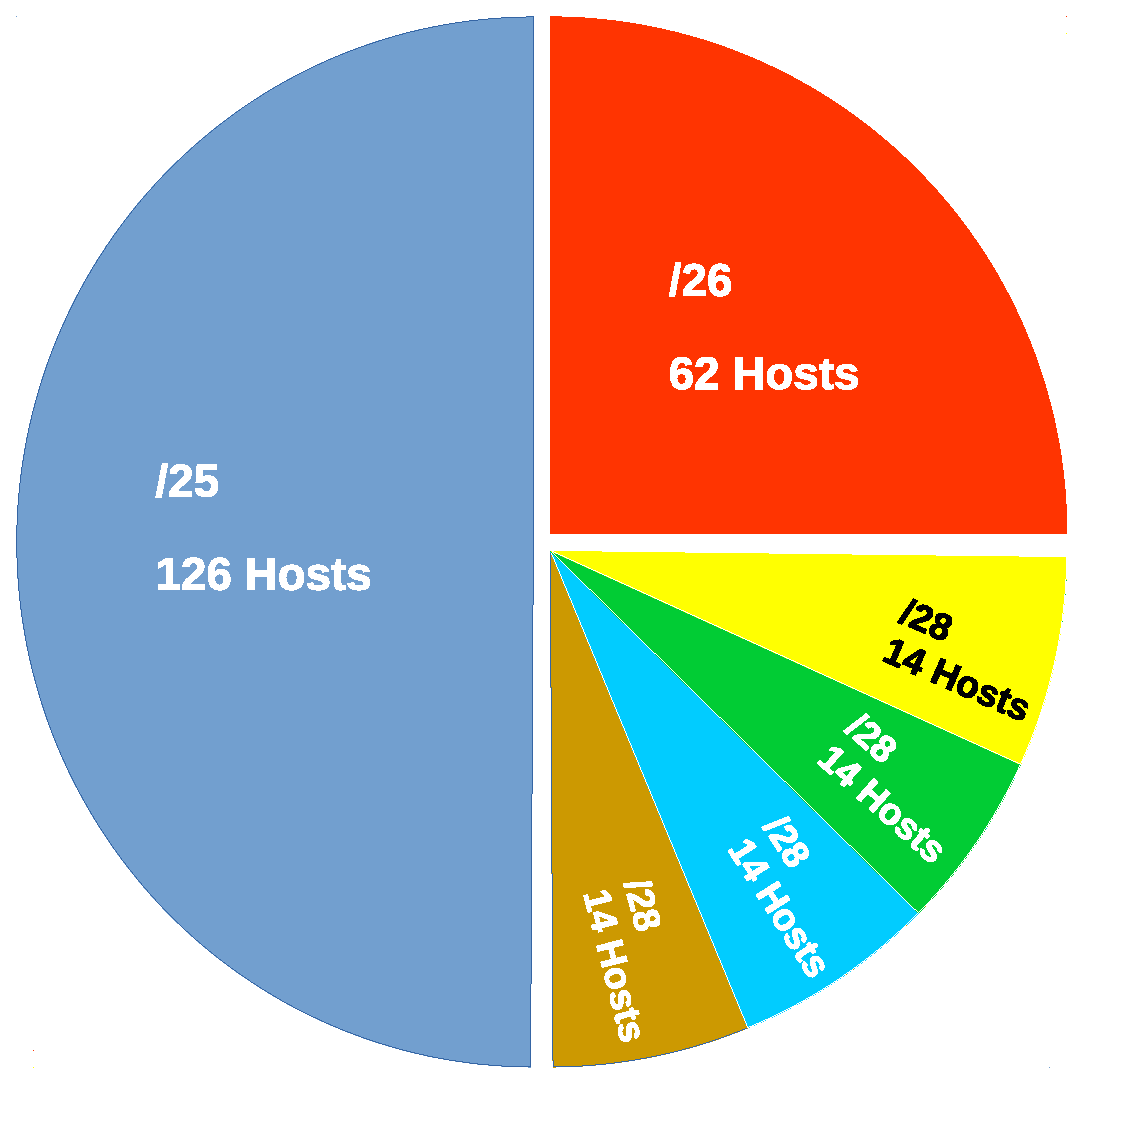
\includegraphics[width=0.55\textwidth]{images/chapter3/3-4}
  \caption {\textsl{Υποδικτύωση με VLSM}}
  \label{3-4}
\end{figure}


Στην περίπτωση της υποδικτύωσης που εξετάσαμε στην προηγούμενη ενότητα, έχου\-με επιπλέον και τη δυνατότητα να μοιράσουμε ένα υποδίκτυο σε περισσότερα. Για παράδειγμα φανταστείτε ένα δίκτυο 192.168.0.0/24 δηλ. με 256 διευθύνσεις (254 υπολογιστές). Μπορούμε να το χωρίσουμε σε δύο υποδίκτυα με πρόθεμα /25 και 128 διευθύνσεις το καθένα (126 υπολογιστές). Από τα υποδίκτυα αυτά μπορούμε να επιλέξουμε να χωρίσουμε το ένα σε δύο επιπλέον υποδίκτυα με πρόθεμα /26 και 64 διευθύνσεις (62 υπολογιστές) κ.ο.κ. (δείτε το σχήμα \ref{3-4}). Καθώς έχουμε πολλαπλά υποδίκτυα που προκύπτουν από τον περαιτέρω διαχωρισμό άλλων υποδικτύων (δηλ. υποδικτύωση υποδικτύων), οι μάσκες που χρησιμοποιούμε έχουν μεταξύ τους διαφορετικό μήκος και ονομάζονται \emph{VLSM, Variable Length Subnet Masking, Μεταβλητού Μήκους Μάσκες Υποδικτύωσης}.